\documentclass[%
pdf,
%nocolorBG,
colorBG,
slideColor,
%slideBW,
%draft,
%frames
%azure
%contemporain
%nuancegris
%troispoints
%lignesbleues
%darkblue
%alienglow
%autumn
]{prosper}
\usepackage{pifont, amsmath, multicol}
%\usepackage{wrapfig,subfigure}
\usepackage{color}
%\usepackage{floatflt}
\usepackage{epsfig}
\usepackage{pifont}
%\usepackage[francais]{babel}
\usepackage[T1]{fontenc}
\usepackage[latin1]{inputenc}
%\catcode`\�=\active
%\catcode`\�=\active
%\def�{\og\ignorespaces}%
%\def�{{\fg}}%

\newcommand{\spacer}{\rule[-3mm]{0mm}{8mm}}
\newtheorem{theorem}{Theorem}
\newtheorem{definition}[theorem]{Definition}
\newtheorem{conjecture}[theorem]{Conjecture}
\newtheorem{corollary}[theorem]{Corollary}
\newtheorem{problem}[theorem]{Problem}
\newtheorem{lemma}{Lemma}
\newtheorem{claim}[theorem]{Claim}
\newtheorem{remark}[theorem]{Remark}
\newtheorem{proposition}[theorem]{Proposition}


\newcommand{\RR}{\ensuremath{\mathbb{R}}}
\newcommand{\NN}{\ensuremath{\mathbb{N}}}
\newcommand{\QQ}{\ensuremath{\mathbb{Q}}}
\newcommand{\CC}{\ensuremath{\mathbb{C}}}
\newcommand{\ZZ}{\ensuremath{\mathbb{Z}}}
\newcommand{\TT}{\ensuremath{\mathbb{T}}}

\def\QuotS#1#2{\leavevmode\kern-.0em\raise.2ex\hbox{$#1$}\kern-.1em/\kern-.1em\lower.25ex\hbox{$#2$}}


\title{\Huge \textcolor{blue}{Goldberg-Coxeter construction}\\[3mm]
\textcolor{blue}{for $3$- or $4$-valent plane graphs}}
\author{
\textcolor{red}{\Large Mathieu Dutour}\\[2mm]
\textcolor{red}{\large ENS/CNRS, Paris and Hebrew University, Jerusalem}\\[2mm]
\textcolor{red}{\Large Michel Deza}\\[2mm]
\textcolor{red}{\large ENS/CNRS, Paris and ISM, Tokyo}
}
\slideCaption{}

\date{}



\begin{document}
\maketitle





\overlays{4}{
\begin{slide}{Goldberg-Coxeter for the Cube}
\onlySlide*{1}{\begin{center}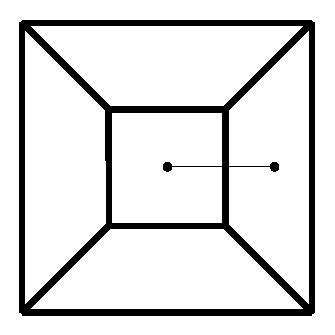
\epsfig{file=GOLDBERGpicture/Cube1_0-sec.eps,width=70mm}\end{center}}%
\onlySlide*{2}{\begin{center}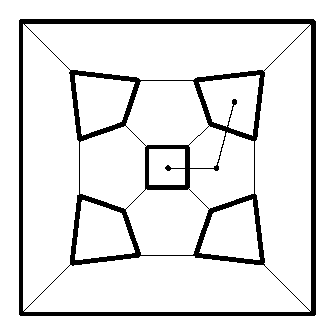
\epsfig{file=GOLDBERGpicture/Cube1_1-sec.eps,width=70mm}\end{center}}%
\onlySlide*{3}{\begin{center}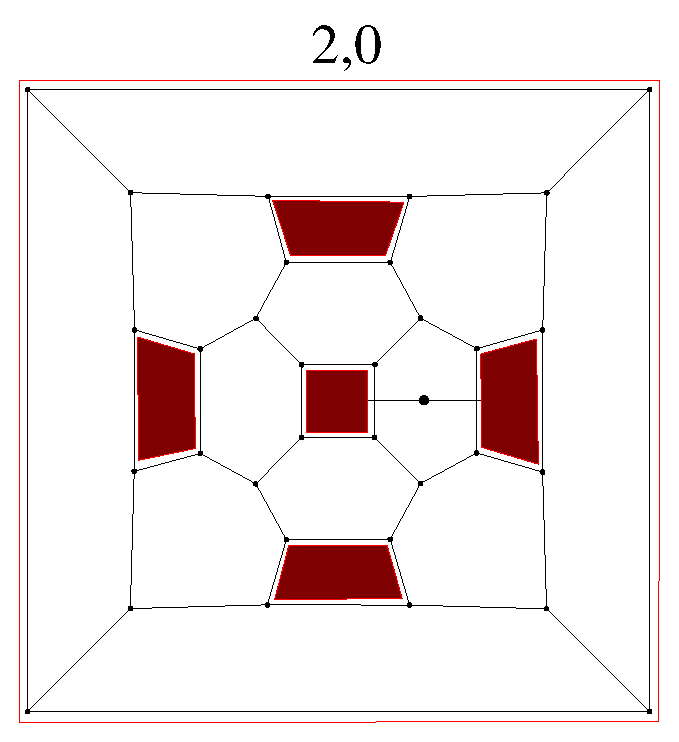
\epsfig{file=GOLDBERGpicture/Cube2_0-sec.eps,width=70mm}\end{center}}%
\onlySlide*{4}{\begin{center}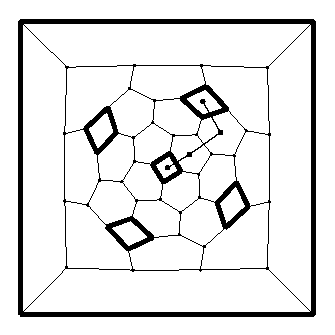
\epsfig{file=GOLDBERGpicture/Cube2_1-sec.eps,width=70mm}\end{center}}%
%\onlySlide*{5}{\begin{center}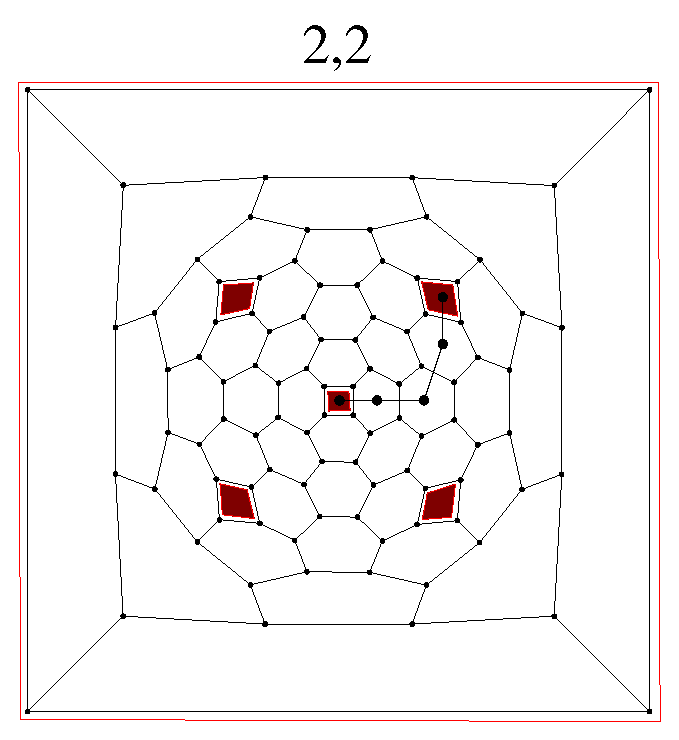
\epsfig{file=GOLDBERGpicture/Cube2_2-sec.eps,width=70mm}\end{center}}%

\end{slide}
}
















%%%%%%%%%%%%%%%   Slide synonyms
\overlays{5}{
\begin{slide}{History}

\onlySlide*{1}{{\bf Mathematics}: construction of planar graphs
\begin{center}
\begin{tabular}{p{10cm}}
M. Goldberg, {\em A class of multisymmetric polyhedra}, Tohoku Math. Journal, {\bf 43} (1937) 104--108.
\end{tabular}
\end{center}
Objective was to maximize the interior volume of the polytope, i.e. to find $3$-dimensional analogs of regular polygons.

\vspace{0.3cm}

\ding{224} search of equidistributed systems of points on the sphere for application to Numerical Analysis.

%\begin{equation*}
%4_n=\left\{\begin{array}{c}
%$3$-\mbox{valent~plane~graphs~with}\\
%$4$\mbox{~or~}$6$\mbox{~gonal~faces}
%\end{array}\right\}
%\end{equation*}
%{\em Goldberg theorem}: All graphs $4_n$ of symmetry $O$ or $O_h$ are obtained by his construction from the Cube.
}%
\onlySlide*{2}{{\bf Biology}: explanation of structure of icosahedral viruses
\begin{center}
\begin{tabular}{p{10cm}}
D.Caspar and A.Klug, {\em Physical Principles in the Construction of Regular Viruses},  Cold Spring Harbor Symp. Quant. Biol., {\bf 27} (1962) 1-24.
\end{tabular}
\end{center}
\begin{center}
\begin{tabular}{|c|c|c|}
\hline
$(k,l)$ & symmetry & capsid of virion\\
\hline
$(1,0)$ & $I_h$ & {\it gemini virus} \\
$(2,0)$ & $I_h$ & {\it hepathite B} \\
$(2,1)$ & $I$, laevo & {\it HK97, rabbit papilloma virus} \\
$(3,1)$ & $I$, laevo & {\it rotavirus} \\
$(4,0)$ & $I_h$ & {\it herpes virus, varicella} \\
$(5,0)$ & $I_h$ & {\it adenovirus} \\
$(6,3)$? & $I$, laevo & {\it HIV-1}\\
\hline
\end{tabular}
\end{center}
}%
\onlySlide*{3}{{\bf Architecture}: construction of geodesic domes

Patent by Buckminster Fuller
\begin{center}
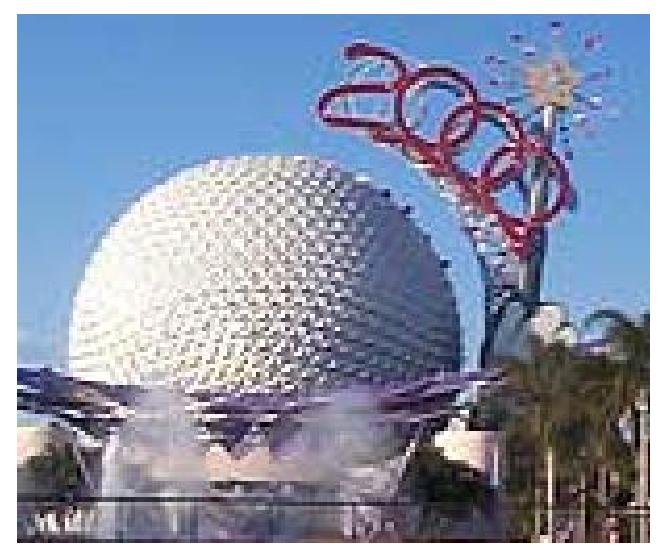
\epsfig{file=GOLDBERGpicture/2000spaceship-modified.eps,width=6.5cm}

EPCOT in Disneyland.
\end{center}
}%
\onlySlide*{4}{{\bf Mathematics}:
\begin{center}
\begin{tabular}{p{10cm}}
H.S.M. Coxeter, {\em Virus macromolecules and geodesic domes}, in {\em A spectrum of mathematics}; ed. by J.C.Butcher, Oxford University Press/Auckland University Press: Oxford, U.K./Auckland New-Zealand, (1971) 98--107.
\end{tabular}
\end{center}
}%
\onlySlide*{5}{{\bf Chemistry}: Buckminsterfullerene $C_{60}$ 

(football, Truncated Icosahedron)
\begin{center}
\begin{tabular}{p{10cm}}
Kroto, Kurl, Smalley (Nobel prize 1996) synthetized in 1985 a new molecule, whose graph is $GC_{1,1}(Dodecahedron)$.

Osawa constructed theoretically $C_{60}$ in 1984.
\end{tabular}
\begin{minipage}{5.5cm}
\centering
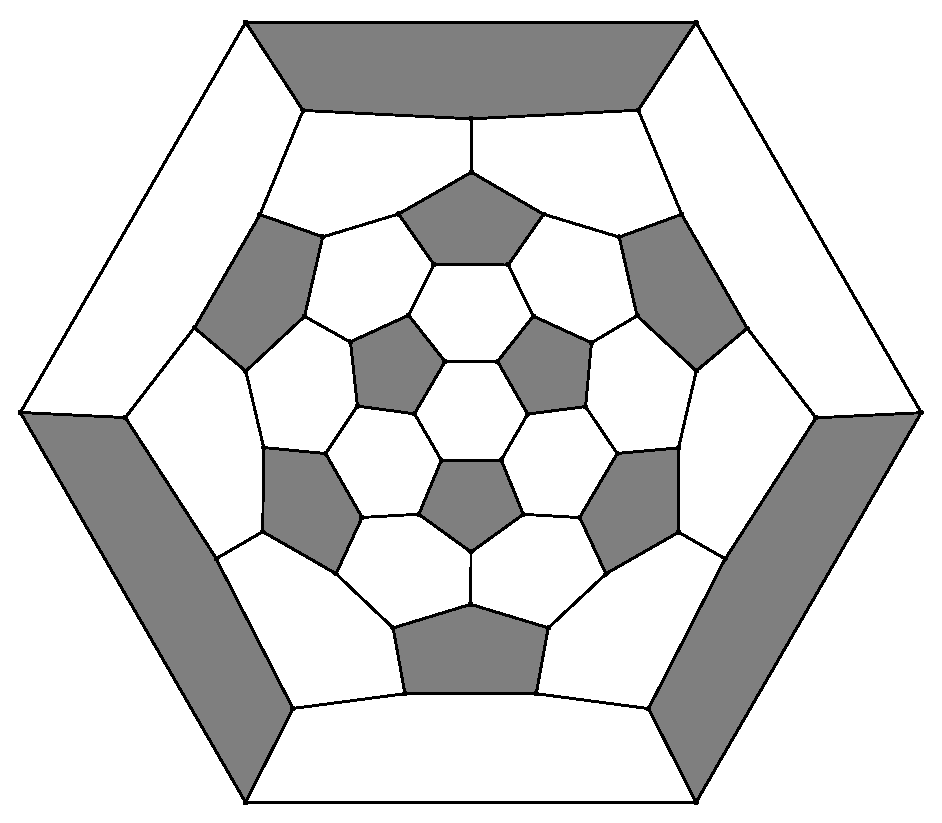
\epsfig{file=GOLDBERGpicture/TruncatedIcosahedronSec.eps,width=50mm}
\end{minipage}
\begin{minipage}{5.5cm}
\centering
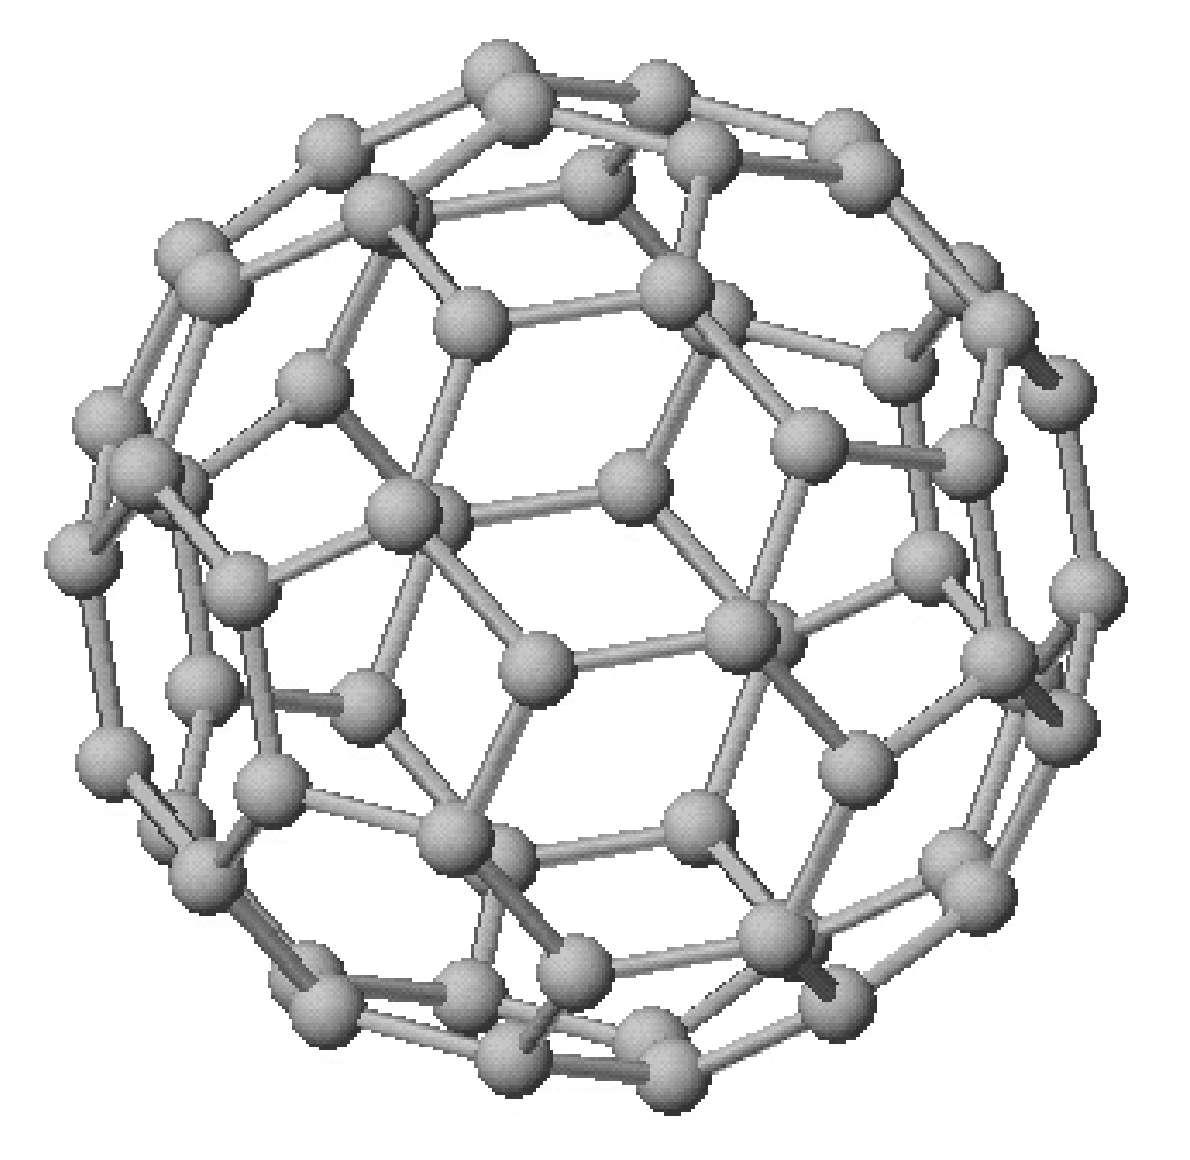
\epsfig{file=GOLDBERGpicture/c60Sec.ps,width=50mm}
\end{minipage}



\end{center}
}%
\end{slide}
}











%\maketitle
%\begin{slide}{PLAN}
%\renewcommand{\theenumi}{\textcolor{blue}{\Roman{enumi}}}
%\renewcommand{\labelenumi}{\theenumi.}
%\renewcommand{\theenumii}{\textcolor{blue}{\alph{enumii}}}
%\renewcommand{\labelenumii}{\theenumii.}
%
%\vspace{1.5cm}
%
%\begin{enumerate}
%\item \textcolor{red}{Zigzags and Central circuits}\\[0.5cm]
%
%\item \textcolor{red}{The Goldberg-Coxeter construction}\\[0.5cm]
%
%\item \textcolor{red}{The $(k,l)$-product}
%
%\end{enumerate}
%
%\end{slide}




%%%%%%%%%%%%%%%%%%%% Slide presentation
\begin{slide}{}
\begin{center}
{\Huge 
\begin{tabular*}{6cm}{c}
\\[-0.5cm]
\textcolor{blue}{I. }\textcolor{red}{ZigZags}\\
\textcolor{red}{and}\\
\textcolor{red}{central circuits}
\end{tabular*}
}
\end{center}
\end{slide}


%%%%%%%%%%%%%%   Central circuits
\overlays{6}{
\begin{slide}{Central circuits}
\onlySlide*{1}{\begin{center}\epsfig{file=GOLDBERGpicture/CentralCircuitSample1.eps,width=11cm}\end{center}}%
\onlySlide*{2}{\begin{center}\epsfig{file=GOLDBERGpicture/CentralCircuitSample2.eps,width=11cm}\end{center}}%
\onlySlide*{3}{\begin{center}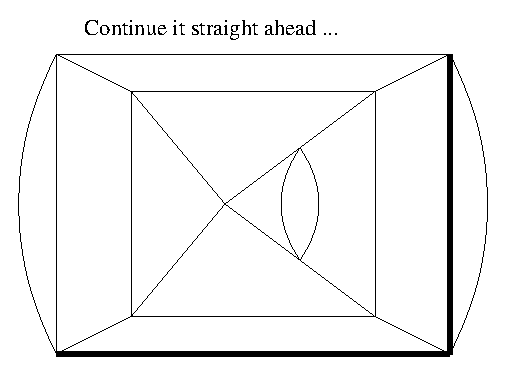
\epsfig{file=GOLDBERGpicture/CentralCircuitSample3.eps,width=11cm}\end{center}}%
\onlySlide*{4}{\begin{center}\epsfig{file=GOLDBERGpicture/CentralCircuitSample4.eps,width=11cm}\end{center}}%
\onlySlide*{5}{\begin{center}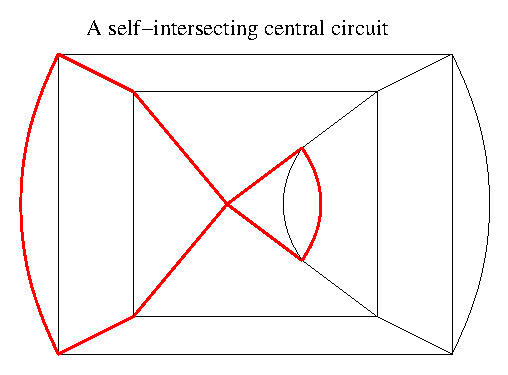
\epsfig{file=GOLDBERGpicture/CentralCircuitSample5.eps,width=11cm}\end{center}}%
\onlySlide*{6}{\begin{center}\epsfig{file=GOLDBERGpicture/CentralCircuitSample6.eps,width=9.8cm}\end{center}}%

\end{slide}
}


%ZIGZAGpicture/
\overlays{6}{
\begin{slide}{Zig Zags}
\onlySlide*{1}{\begin{center}\epsfig{file=ZIGZAGpicture/ZigZagSample1.eps,width=11cm}\end{center}}%
\onlySlide*{2}{\begin{center}\epsfig{file=ZIGZAGpicture/ZigZagSample2.eps,width=11cm}\end{center}}%
\onlySlide*{3}{\begin{center}\epsfig{file=ZIGZAGpicture/ZigZagSample3.eps,width=11cm}\end{center}}%
\onlySlide*{4}{\begin{center}\epsfig{file=ZIGZAGpicture/ZigZagSample4.eps,width=11cm}\end{center}}%
\onlySlide*{5}{\begin{center}\epsfig{file=ZIGZAGpicture/ZigZagSample5.eps,width=11cm}\end{center}}%
\onlySlide*{6}{\begin{center}\epsfig{file=ZIGZAGpicture/ZigZagSample6sharp.eps,width=9.8cm}\end{center}}%
\end{slide}
}





\begin{slide}{Notations}
\begin{itemize}
\item \textcolor{red}{ZC-circuit} stands for ``zigzag or central circuit'' in $3$- or $4$-valent plane graphs.
\vspace{1cm}


\item The \textcolor{red}{length} of a ZC-circuit is the number of its edges.
\vspace{1cm}


\item The \textcolor{red}{ZC-vector} of a $3$- or $4$-valent plane graph $G_0$ is the vector $\dots, c_k^{m_k}, \dots$ where $m_k$ is the number of ZC-circuits of length $c_k$.
\vspace{1cm}

%\item[\ding{108}] A graph is ZC-transitive if its group of automorphism is transitive on the set of ZC-circuits

\end{itemize}

\end{slide}



%%%%%%%%%%%%%  operators



%%%%%%%%%%%%%%%%%%%% Slide presentation
\begin{slide}{}
\begin{center}
{\Huge 
\begin{tabular*}{8cm}{c}
\\[-0.5cm]
\textcolor{blue}{II. }\textcolor{red}{Goldberg-Coxeter}\\
\textcolor{red}{construction}
\end{tabular*}
}
\end{center}
\end{slide}

%%%%%%%%%%%%%%%%%%%%  the construction
\begin{slide}{The construction}
\begin{itemize}
\item Take a $3$- or $4$-valent plane graph $G_0$. The graph $G_0^{*}$ is formed of triangles or squares.
\item Break the triangles or squares into pieces:
\end{itemize}
\begin{center}
\epsfig{file=GOLDBERGpicture/GoldbergBreakdown.eps,width=115mm}
\end{center}

\end{slide}


%%%%%%%%%%%%%%%%%%% sequel of construction
\overlays{4}{
\begin{slide}{Gluing the pieces}
\fromSlide{1}{
\begin{itemize}
\item Glue the pieces together in a coherent way.
\item We obtain another \textcolor{red}{triangulation} or \textcolor{red}{quadrangulation} of the plane.
\end{itemize}
}%
\onlySlide*{1}{
\begin{center}
\begin{minipage}{5.5cm}
\centering
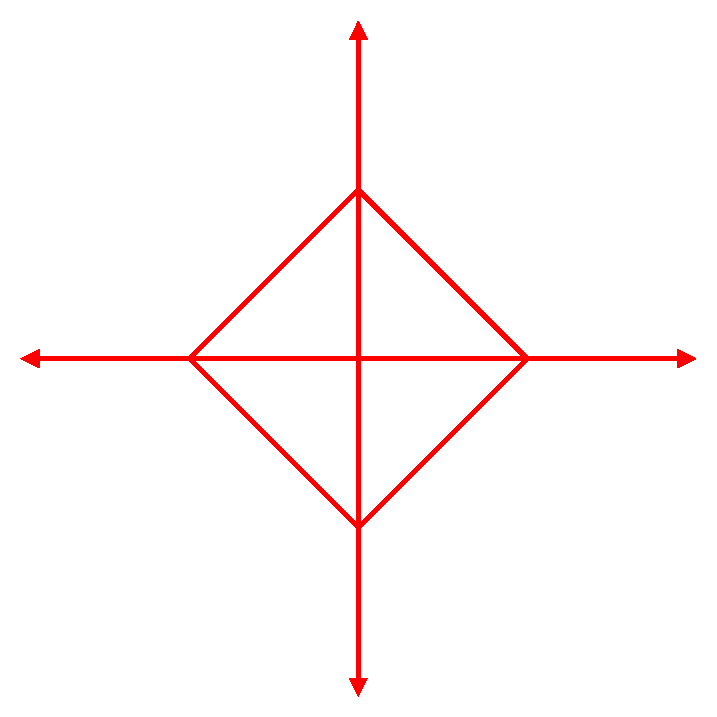
\epsfig{file=GOLDBERGpicture/SimpleCaseOfConstruction3-valent1.eps,width=50mm}\par
Case $3$-valent
\end{minipage}
\begin{minipage}{5.5cm}
\centering
\epsfig{file=GOLDBERGpicture/SimpleCaseOfConstruction4-valent1.eps,width=50mm}\par
Case $4$-valent
\end{minipage}
\end{center}
}%
\onlySlide*{2}{
\begin{center}
\begin{minipage}{5.5cm}
\centering
\epsfig{file=GOLDBERGpicture/SimpleCaseOfConstruction3-valent2.eps,width=50mm}\par
$(3,0)$: $3$-valent
\end{minipage}
\begin{minipage}{5.5cm}
\centering
\epsfig{file=GOLDBERGpicture/SimpleCaseOfConstruction4-valent2.eps,width=50mm}\par
$(3,0)$: $4$-valent
\end{minipage}
\end{center}
}%
\onlySlide*{3}{
\begin{center}
\centering
\epsfig{file=GOLDBERGpicture/MergingBreakdown1.eps,width=50mm}
\end{center}
}%
\onlySlide*{4}{
\begin{center}
\centering
\epsfig{file=GOLDBERGpicture/MergingBreakdown2.eps,width=50mm}
\end{center}
}%






\end{slide}
}








\begin{slide}{Final steps}

\begin{itemize}
\item Go to the dual and obtain a $3$- or $4$-valent plane graph, which is denoted $GC_{k,l}(G_0)$ and called ``Goldberg-Coxeter construction''.
\item The construction works for any $3$- or $4$-valent map on \textcolor{red}{oriented surface}.
\end{itemize}
\vspace{-2mm}
\begin{center}
\begin{minipage}[t]{7cm}
\centering
\epsfxsize=6cm
\epsffile{GOLDBERGpicture/eberhardSec.eps}\par
\end{minipage}
\begin{minipage}[t]{3cm}
\centering
\epsfxsize=2.7cm
\epsffile{GOLDBERGpicture/C80Sec.eps}\par
\end{minipage}
\end{center}
\begin{center}
Operation $GC_{2,0}$
\end{center}




\end{slide}









%%%%%%%%%%%% an example at length.

\overlays{7}{
\begin{slide}{Example of $GC_{3,2}(Octahedron)$}
%\onlySlide*{1}{\begin{center}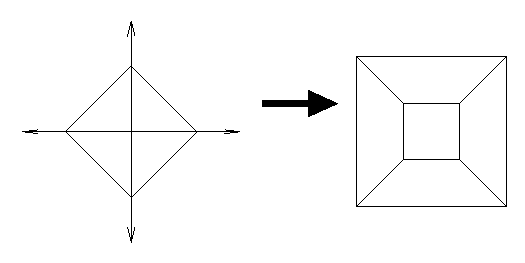
\epsfig{file=Octahedron.eps,width=80mm}\end{center}}%
\onlySlide*{1}{\begin{center}\epsfig{file=GOLDBERGpicture/OctahedronSec.eps,width=100mm}\end{center}}%
%\onlySlide*{2}{\begin{center}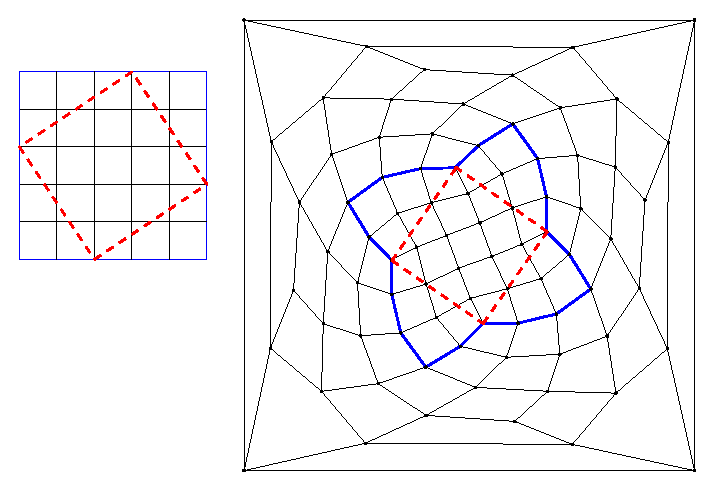
\epsfig{file=dualPL32sec.eps,width=80mm}\end{center}}%
\onlySlide*{2}{\begin{center}\epsfig{file=GOLDBERGpicture/NewDualPL32secNr1.eps,width=107mm}\end{center}}%
\onlySlide*{3}{\begin{center}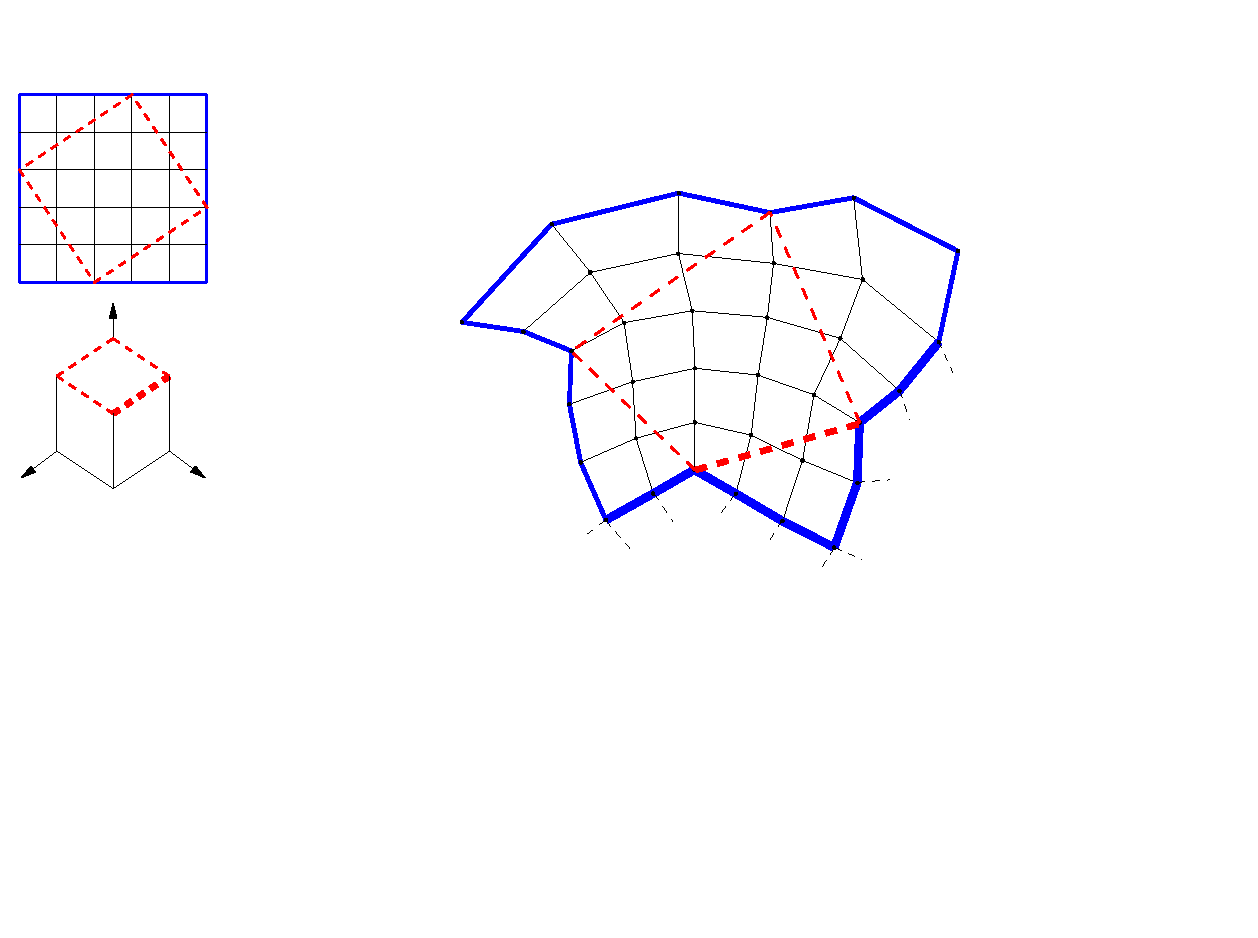
\epsfig{file=GOLDBERGpicture/NewDualPL32secNr1_2.eps,width=107mm}\end{center}}%
\onlySlide*{4}{\begin{center}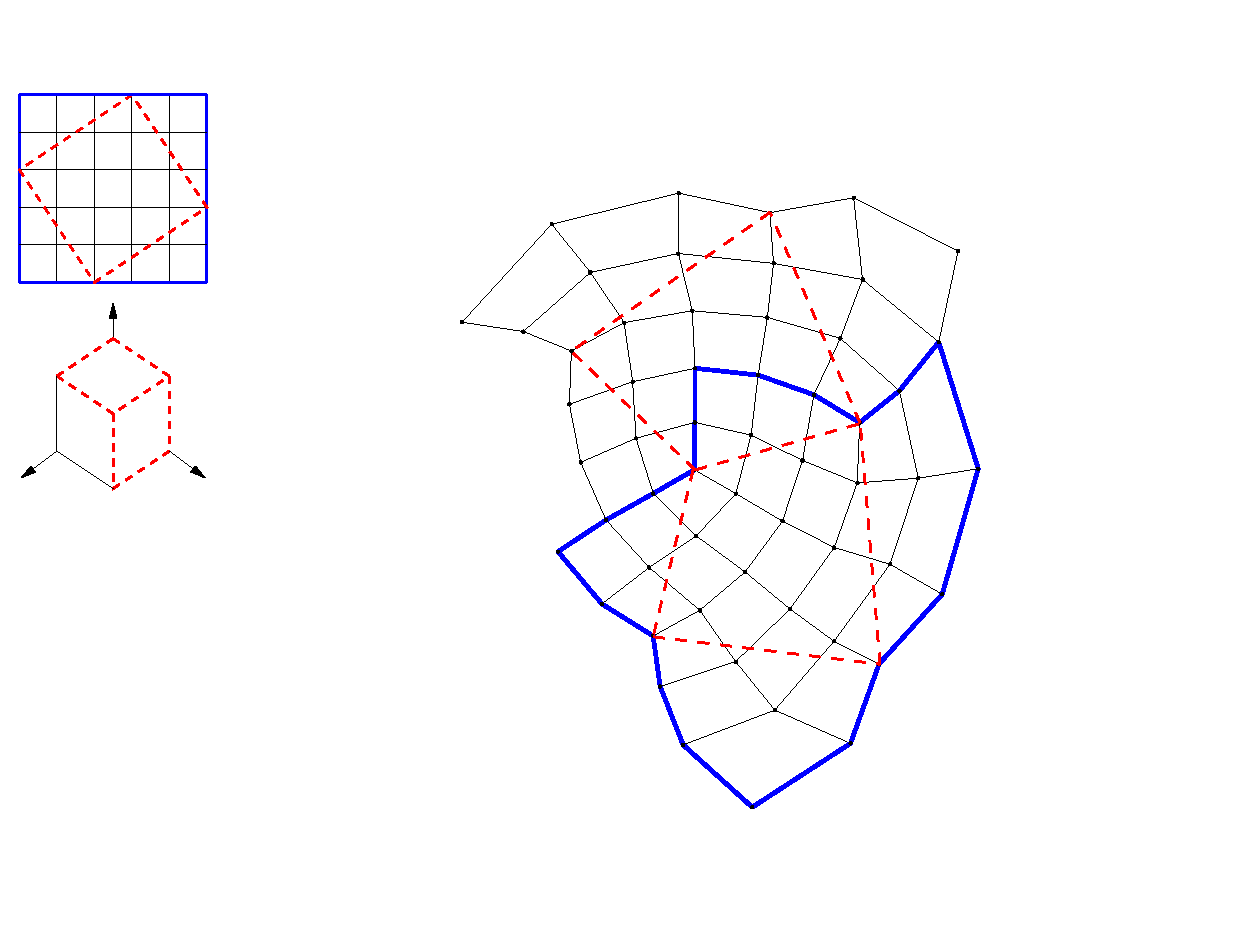
\epsfig{file=GOLDBERGpicture/NewDualPL32secNr2.eps,width=107mm}\end{center}}%
\onlySlide*{5}{\begin{center}\epsfig{file=GOLDBERGpicture/NewDualPL32secNr3.eps,width=107mm}\end{center}}%
\onlySlide*{6}{\begin{center}\epsfig{file=GOLDBERGpicture/NewDualPL32secNr4.eps,width=107mm}\end{center}}%
%\onlySlide*{3}{\begin{center}\epsfig{file=dualPL32secSquares.eps,width=80mm}\end{center}}%
%\onlySlide*{6}{\begin{center}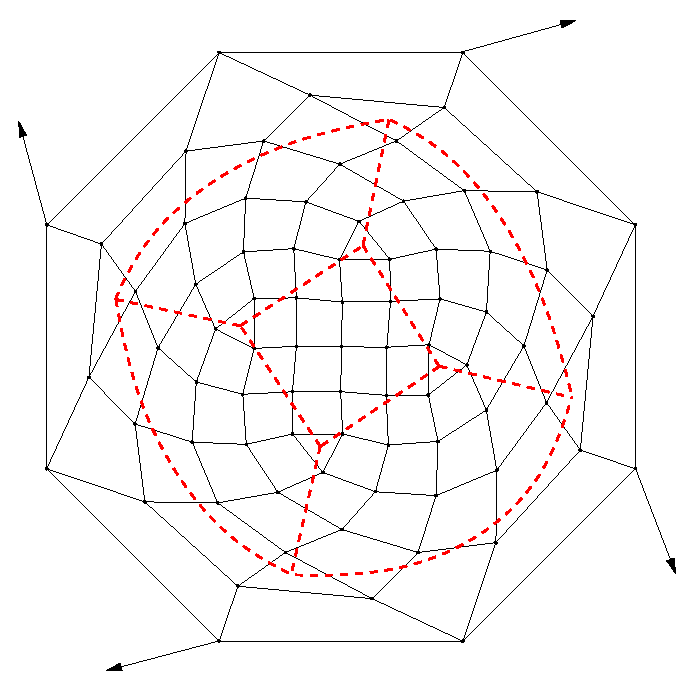
\epsfig{file=nPL32thi.eps,width=80mm}\end{center}}%
\onlySlide*{7}{\begin{center}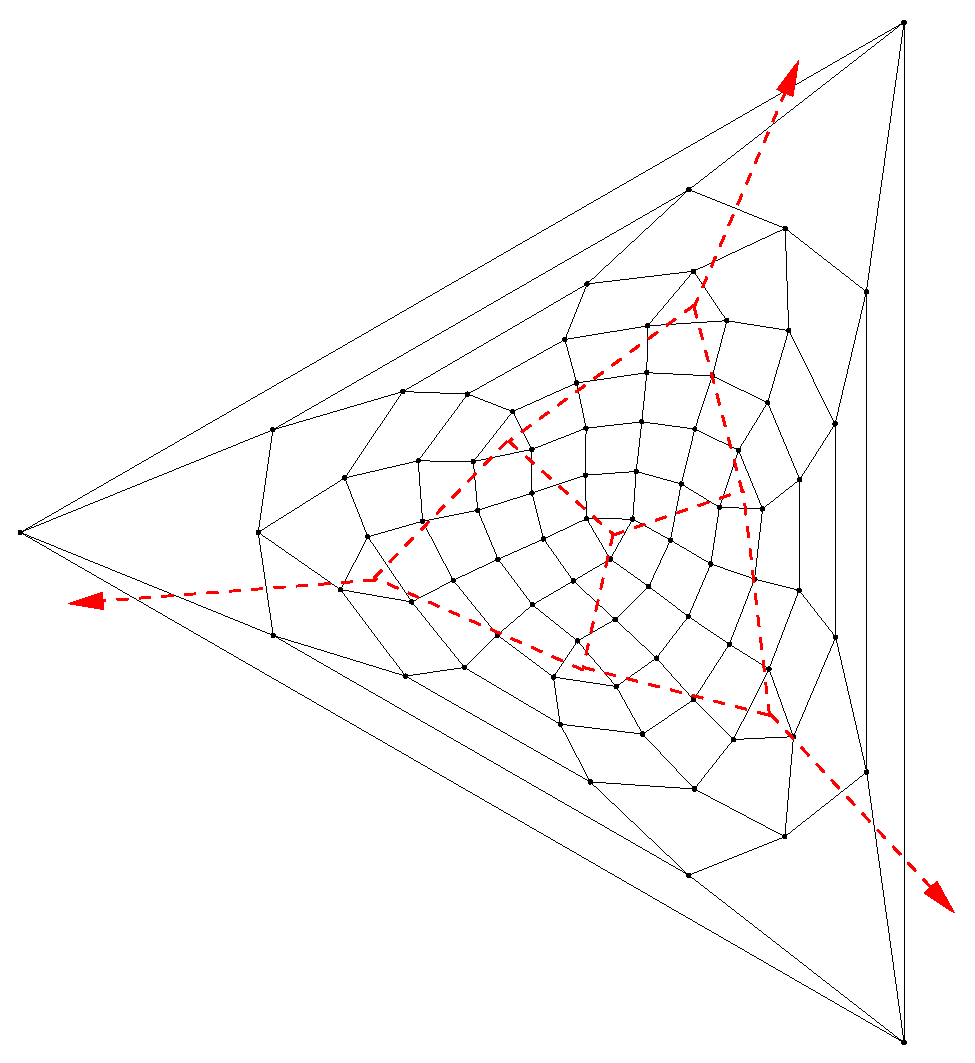
\epsfig{file=GOLDBERGpicture/3foldViewPL32sec.eps,width=70mm}\end{center}}%
\end{slide}
}






\begin{slide}{Properties}
\vspace{-3mm}
\begin{itemize}
\item One associates \textcolor{red}{$z=k+le^{i\frac{\pi}{3}}$(Eisenstein integer)} or \textcolor{red}{$z=k+li$(Gaussian integer)} to the pair $(k,l)$ in $3$- or $4$-valent case.

\item If one writes \textcolor{red}{$GC_{z}(G_0)$} instead of $GC_{k,l}(G_0)$, then one has:
\begin{equation*}
\begin{array}{rcl}
GC_{z}(GC_{z'}(G_0))  &=&GC_{zz'}(G_0)
%GC_{\overline{z}}(G_0)&=&GC_{z}(\overline{G_0})
\end{array}
\end{equation*}
%with $\overline{G_0}$ the symmetric on a plane of $G_0$.

%\item[\ding{108}] $GC_{1,0}(G_0)=G_0$
\item If $G_0$ has $n$ vertices, then $GC_{k,l}(G_0)$ has 
\begin{center}
\begin{tabular}{rcl}
$n(k^2+kl+l^2)=n|z|^2$ vertices &if& $G_0$ is $3$-valent,\\
$n(k^2+l^2)=n|z|^2$ vertices &if& $G_0$ is $4$-valent.
\end{tabular}
\end{center}
\item If $G_0$ has a plane of symmetry, we reduce to $0\leq l\leq k$.
\item $GC_{k,l}(G_0)$ has all rotational symmetries of $G_0$ and all symmetries if $l=0$ or $l=k$.
\end{itemize}

\end{slide}



%%%%%%%%%%% medial and leapfrog
\overlays{3}{
\begin{slide}{The case $(k,l)=(1,1)$}
\onlySlide*{1}{
\begin{center}
\begin{minipage}{5.5cm}
\centering
\epsfig{file=GOLDBERGpicture/ExampleLeapFrog1.eps,width=50mm}\par
Case $3$-valent
\end{minipage}
\begin{minipage}{5.5cm}
\centering
\epsfig{file=GOLDBERGpicture/ExampleMedial1.eps,width=50mm}\par
\vspace{0.9cm}
Case $4$-valent
\end{minipage}
\end{center}
}
\onlySlide*{2}{
\begin{center}
\begin{minipage}{5.5cm}
\centering
\epsfig{file=GOLDBERGpicture/ExampleLeapFrog2.eps,width=50mm}\par
Case $3$-valent
\end{minipage}
\begin{minipage}{5.5cm}
\centering
\epsfig{file=GOLDBERGpicture/ExampleMedial2.eps,width=50mm}\par
\vspace{0.9cm}
Case $4$-valent
\end{minipage}
\end{center}
}
\onlySlide*{3}{
\begin{center}
\begin{minipage}{5.5cm}
\centering
\epsfig{file=GOLDBERGpicture/ExampleLeapFrog3.eps,width=50mm}\par
Case $3$-valent\par
$GC_{1,1}$ is called \textcolor{red}{leapfrog}
(=Truncation of the dual)
\end{minipage}
\begin{minipage}{5.5cm}
\centering
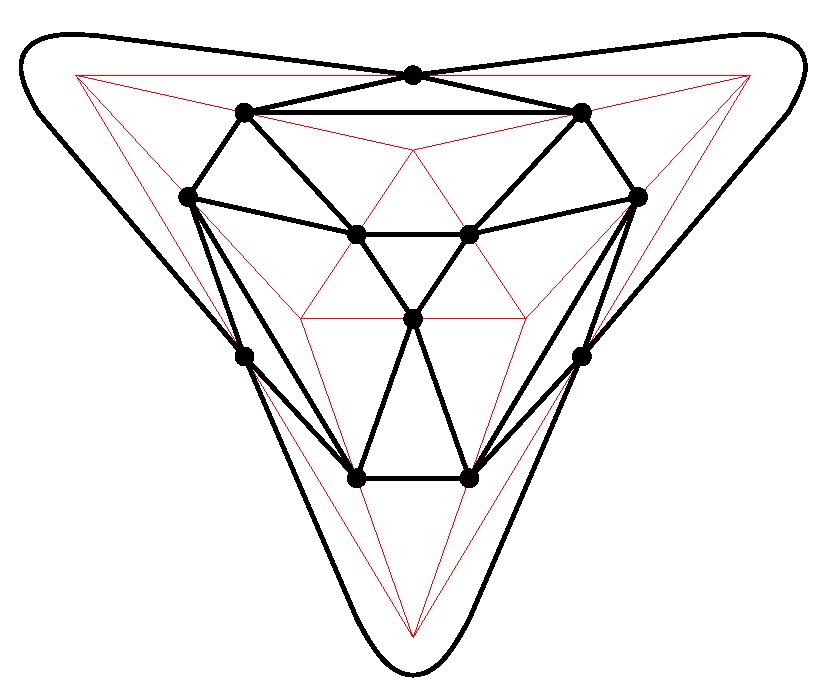
\epsfig{file=GOLDBERGpicture/ExampleMedial3.eps,width=50mm}\par
\vspace{0.9cm}
Case $4$-valent\par
$GC_{1,1}$ is called \textcolor{red}{medial}\par
\textcolor{white}{Bonjour}
\end{minipage}
\end{center}
}
\end{slide}
}


%%%%%%%%%%%%%%   Goldberg Theorem's
\begin{slide}{Goldberg Theorem}
\begin{itemize}
\item \textcolor{red}{$q_n$} is the class of $3$-valent plane graphs having only $q$- and $6$-gonal faces.
\item The class of $4$-valent plane graphs having only $3$- and $4$-gonal faces is called \textcolor{red}{Octahedrites}.
\end{itemize}



\begin{center}
{\small
\begin{tabular}{|c|c|c|c|}
\hline
Class&             &Groups    &Construction\\
\hline
$3_n$&$p_3=4$      &$T$, $T_d$&$GC_{k,l}(\mbox{Tetrahedron})$\\
$4_n$&$p_4=6$      &$O$, $O_h$&$GC_{k,l}(\mbox{Cube})$\\
$4_n$&$p_4=6$      &$D_6$, $D_{6h}$&$GC_{k,l}(\mbox{Prism}_6)$\\
$5_n$&$p_5=12$     &$I$, $I_h$&$GC_{k,l}(\mbox{Dodecahedron})$\\
Octahedrites&$p_3=8$&$O$, $O_h$&$GC_{k,l}(\mbox{Octahedron})$\\
\hline
\end{tabular}
}
\end{center}




\end{slide}






%%%%%%%%%%%%%%  k-inflation theorem
\overlays{3}{
\begin{slide}{The special case $GC_{k,0}$}
\fromSlide{1}{
\begin{itemize}
\item Any ZC-circuit of $G_0$ corresponds to \textcolor{red}{$k$ ZC-circuits} of $GC_{k,0}(G_0)$ with length \textcolor{red}{multiplied by $k$}.
\item If the ZC-vector of $G_0$ is $\dots, c_l^{m_l}, \dots$, then the ZC-vector of $GC_{k,0}(G_0)$ is \textcolor{red}{$\dots, (kc_l)^{km_l}, \dots$}.
\end{itemize}
}
\onlySlide*{1}{
\begin{center}
\begin{minipage}{5.5cm}
\centering
\epsfig{file=GOLDBERGpicture/Cube10Sec.eps,width=50mm}
\end{minipage}
\begin{minipage}{5.5cm}
\centering
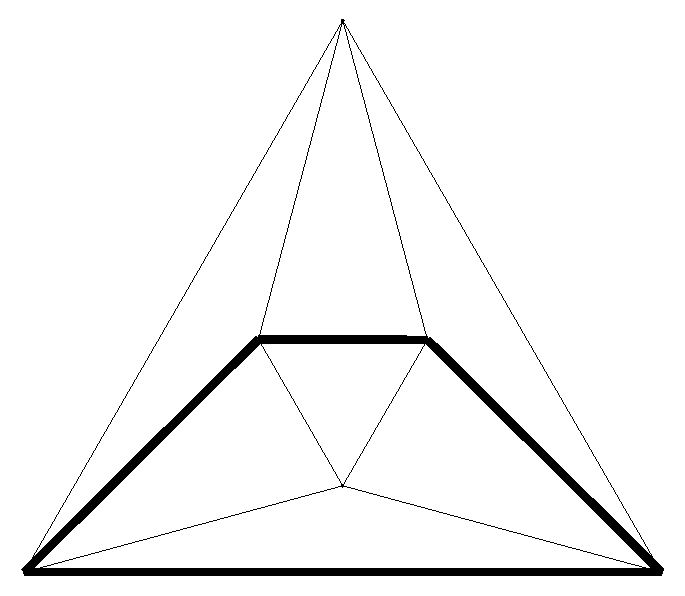
\epsfig{file=GOLDBERGpicture/Octahedron10Sec.eps,width=50mm}
\end{minipage}
\end{center}
}%
\onlySlide*{2}{
\begin{center}
\begin{minipage}{5.5cm}
\centering
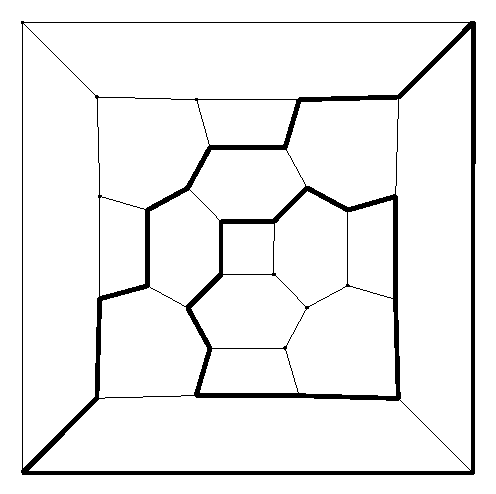
\epsfig{file=GOLDBERGpicture/Cube20Sec.eps,width=50mm}
\end{minipage}
\begin{minipage}{5.5cm}
\centering
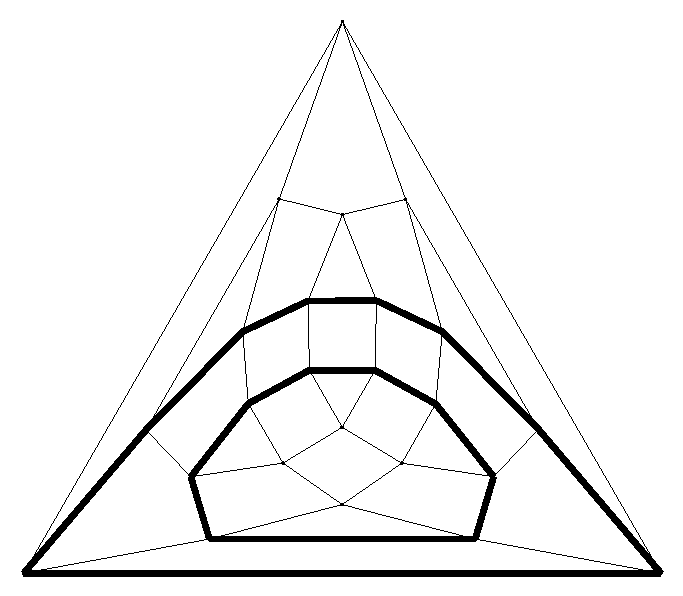
\epsfig{file=GOLDBERGpicture/Octahedron20Sec.eps,width=50mm}
\end{minipage}
\end{center}
}%
\onlySlide*{3}{
\begin{center}
\begin{minipage}{5.5cm}
\centering
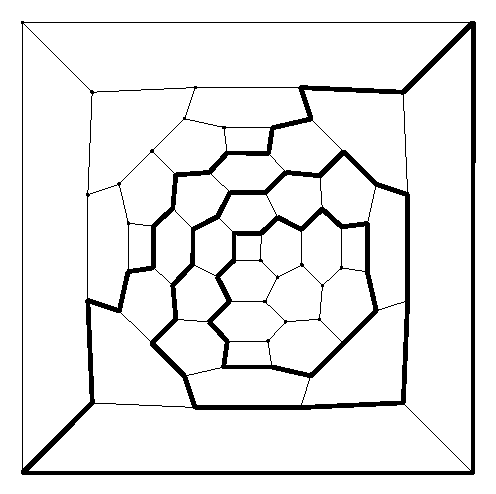
\epsfig{file=GOLDBERGpicture/Cube30Sec.eps,width=50mm}
\end{minipage}
\begin{minipage}{5.5cm}
\centering
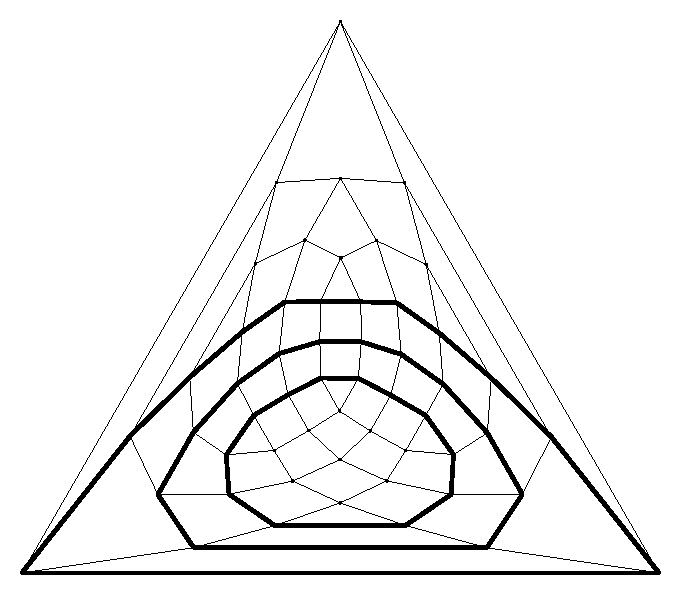
\epsfig{file=GOLDBERGpicture/Octahedron30Sec.eps,width=50mm}
\end{minipage}
\end{center}
}%

\end{slide}
}




%%%%%%%%%%%%%%%%%%%% The (k,l)-product
\begin{slide}{}
\begin{center}
{\Huge 
\begin{tabular*}{6cm}{c}
\\[-0.5cm]
\textcolor{blue}{III. }\textcolor{red}{The}\\
\textcolor{red}{$(k,l)$-product}
\end{tabular*}
}
\end{center}
\end{slide}





%%%%%%%%%%%%%%%%%%%%   the mapping phi_{k,l}

\begin{slide}{The mapping $\phi_{k,l}$}
\textcolor{red}{We always assume $gcd(k,l)=1$}
\begin{equation*}
\left\lbrace\begin{array}{rcl}
\textcolor{red}{\phi_{k,l}}:\{1,\dots, k+l\}  &\rightarrow   &\{1,\dots, k+l\}\\
u                             &\mapsto       &\left\lbrace\begin{array}{rcl}
u+l  &\mbox{~if~}   &u\in \{1,\dots, k\}\\
u-k  &\mbox{~if~}   &u\in \{k+1,\dots, k+l\}\\
\end{array}\right.
\end{array}\right.
\end{equation*}
is bijective and periodic with period $k+l$.

\vspace{0.3cm}

\textcolor{blue}{Example:} Case $k=5$, $l=2$:
\begin{equation*}
\begin{array}{l}
\phi^{(s)}(1)=1, 3, 5, 7, 2, 4, 6, 1, \dots\\
\mbox{operations:} (+2), (+2), (+2), (-5), (+2), (+2), (-5)
\end{array}
\end{equation*}


\end{slide}


\begin{slide}{The $(k,l)$-product}

\begin{itemize}
\item
\begin{definition}(The $(k,l)$-product) 

If $L$ and $R$ are two elements of a group, $k,l\geq 0$ and $gcd(k,l)=1$; we define\\
$(p_0, \dots, p_{k+l})$ by $p_0=1$ and $p_{i}=\phi_{k,l}(p_{i-1})$.

Set \textcolor{red}{$S_i=L$} if $p_{i}-p_{i-1}=l$ and \textcolor{red}{$S_i=R$} if $p_{i}-p_{i-1}=-k$; then set
\begin{equation*}
\textcolor{red}{L\odot_{k,l} R=S_{k+l}\dots S_{2}\cdot S_{1}}.
\end{equation*}
By convention, set $L \odot_{1,0} R=L$ and $L\odot_{0,1} R=R$.\\
\end{definition}
For $k=5$, $l=2$, one gets the expression
\begin{equation*}
L\odot_{5,2} R=RLLRLLL
\end{equation*}
\item A similar notion is introduced by Norton (1987) in ``Generalized Moonshine'' for the Monster group.

\end{itemize}
\end{slide}


%%%%%%%%%%%   sequel of (k,l)-product
\begin{slide}{Properties}
\begin{itemize}
\item If $L$ and $R$ commute, $L \odot_{k,l} R=L^k R^l$
\item Euclidean algorithm formula
\begin{equation*}
\left\lbrace\begin{array}{rcrcll}
L\odot_{k,l} R&=&  L   &\odot_{k-ql\mbox{~},\mbox{~}l}&RL^q  &\mbox{if~}k-ql\geq 0\\
L\odot_{k,l} R&=&  R^qL&\odot_{k\mbox{~},\mbox{~} l-qk}&R     &\mbox{if~}l-qk\geq 0
\end{array}\right.
\end{equation*}

\item[\ding{224}] If $L$ and $R$ do not commute, then $L\odot_{k,l} R\not= Id$.

\end{itemize}
\end{slide}


%%%%%%%%%%%%%%%%%%%% The (k,l)-product
\begin{slide}{}
\begin{center}
{\Huge 
\begin{tabular*}{6cm}{c}
\\[-0.5cm]
\textcolor{blue}{IV. }\textcolor{red}{ZC-circuits}\\
\textcolor{red}{in}\\
\textcolor{red}{$GC_{k,l}(G_0)$}
\end{tabular*}
}
\end{center}
\end{slide}





%%%%%%%%%%%%%%%%%  the position mapping 
\overlays{6}{\begin{slide}{Position mapping, $3$-valent case}
\onlySlide*{1}{\begin{center}\epsfig{file=GOLDBERGpicture/PositionMapping3-Valent0-1.eps,width=80mm}\end{center}}%
\onlySlide*{2}{\begin{center}\epsfig{file=GOLDBERGpicture/PositionMapping3-Valent0-2.eps,width=80mm}\end{center}}%
\onlySlide*{3}{\begin{center}\epsfig{file=GOLDBERGpicture/PositionMapping3-Valent1.eps,width=80mm}\end{center}}%
\onlySlide*{4}{\begin{center}\epsfig{file=GOLDBERGpicture/PositionMapping3-Valent2.eps,width=80mm}\end{center}}%
\onlySlide*{5}{\begin{center}\epsfig{file=GOLDBERGpicture/PositionMapping3-Valent3.eps,width=90mm}\end{center}}%
\onlySlide*{6}{\begin{center}\epsfig{file=GOLDBERGpicture/PositionMapping3-Valent4.eps,width=90mm}\end{center}}%

\end{slide}
}


%%%%%%%%%%%%%%%%  Iterating the position mapping


\begin{slide}{Iteration}
\vspace{-3mm}
\begin{itemize}
\item ``Position mapping'' is denoted \textcolor{red}{$PM(\overrightarrow{e}, p)$}=\textcolor{red}{$(\overrightarrow{f}_1, \phi_{k,l}(p))$} or \textcolor{red}{$(\overrightarrow{f}_2, \phi_{k,l}(p))$}
\item $PM^{k+l}(\overrightarrow{e}, 1)$=$(\overrightarrow{e}', 1)$. So, one defines ``Iterated position mapping'' as \textcolor{red}{$IPM(\overrightarrow{e})=\overrightarrow{e}'$}.
\item \textcolor{red}{${\cal DE}$} is the set of directed edges of $G_0^*$. $IPM$ is a permutation of ${\cal DE}$.
\item For every ZC-circuit with pair $(\overrightarrow{e}, 1)$ denote \textcolor{red}{$Ord(ZC)$} the smallest $s>0$, such that $IPM^s(\overrightarrow{e})=\overrightarrow{e}$.
\item[\ding{224}] For any ZC-circuit of $GC_{k,l}(G_0)$ one has:
\begin{tabular}{lll}
${\rm length}(ZC)$=$2(k^2+kl+l^2)Ord(ZC)$& $3$-valent case\\
${\rm length}(ZC)$=$(k^2+l^2)Ord(ZC)$ & $4$-valent case
\end{tabular}



The \textcolor{red}{[ZC]-vector} of $GC_{k,l}(G_0)$ is the vector $\dots, c_k^{m_k}, \dots$ where $m_k$ is the number of ZC-circuits with \textcolor{red}{order} $c_k$.

%If ZC of $GC_{k,l}(G_0)$ is \dots, $c_k^{m_k}$,\dots then \textcolor{red}{[ZC]} of $GC_{k,l}(G_0)$ is \dots, $\{\frac{c_k}{2(k^2+kl+l^2)}\}^{m_k}$,\dots or \dots, $\{\frac{c_k}{k^2+l^2}\}^{m_k}$,\dots.


%\item[\ding{108}] Denote [ZC]=
% the ZC-vector of $GC_{k,l}(G_0)$ with $c_k$ being the length divided by $2(k^2+kl+l^2)$ or $k^2+l^2$.
\end{itemize}
\end{slide}



%%%%%%%%%%%%%%%%%%%%  computation of L and R
\overlays{4}{
\begin{slide}{The mappings $L$ and $R$}
\onlySlide*{1}{
\begin{itemize}

\item \textcolor{red}{$L$} and \textcolor{red}{$R$} are the following permutation of ${\cal DE}$
\begin{equation*}
\textcolor{red}{L:\overrightarrow{e}\rightarrow\overrightarrow{f}_1}
\mbox{~~~~~~~~~~~~~}
\textcolor{red}{R:\overrightarrow{e}\rightarrow\overrightarrow{f}_2}
\end{equation*}
with $\overrightarrow{f}_1$ and $\overrightarrow{f}_2$ being the first and second choice. \textcolor{red}{Example of Cube}
\end{itemize}
\begin{center}
\epsfig{file=GOLDBERGpicture/LRmappings1-octahedron.eps,width=40mm}
\end{center}
}%
\onlySlide*{2}{
\begin{center}
\epsfig{file=GOLDBERGpicture/LRmappings2-directed-edges.eps,width=70mm}
\end{center}
}%
\onlySlide*{3}{
\begin{center}
\epsfig{file=GOLDBERGpicture/LRmappings4-OneCycle.eps,width=70mm}
\end{center}
}%
\onlySlide*{4}{
\begin{center}
\epsfig{file=GOLDBERGpicture/LRmappings6-OtherCycles.eps,width=70mm}
\end{center}
}%
\end{slide}
}









%%%%%%%%%%%%%%%%%%%%  The moving group
\begin{slide}{Moving group and Key Theorem}
\begin{itemize}
\item \textcolor{red}{$Mov(G_0)=\langle L, R\rangle$} is the \textcolor{red}{moving group}

\textcolor{red}{In Cube}: a subgroup of $Sym(24)$.

\item For $u\in Mov(G_0)$, denote \textcolor{red}{$ZC(u)$} the vector $\dots, c_k^{m_k},\dots$ with multiplicities $m_k$ being the \textcolor{red}{half of the number of cycles of length $c_k$} in the permutation $u$ acting on the set ${\cal DE}$.

\textcolor{red}{In Cube}: \textcolor{blue}{$ZC(L)=ZC(R)=3^{4}$}

\item[\ding{224}] \textcolor{red}{Key Theorem} One has for all $3$- or $4$-valent plane graphs $G_0$ and all $k,l\geq 0$

\begin{center}
\textcolor{blue}{$[ZC]-vector\mbox{~of~}GC_{k,l}(G_0)= ZC(L\odot_{k,l} R)$}
\end{center}

\end{itemize}
\end{slide}











%%%%%%%%%%%   sequel of (k,l)-product
%\begin{slide}{Fundamental Theorem}
%\begin{enumerate}
%\end{enumerate}
%\end{slide}







%%%%%% the case of cube
\begin{slide}{Solution of the Cube case}
\begin{itemize}
\item $L$ and $R$ do not commute \ding{224} $L\odot_{k,l} R\not= Id$.
\item $Mov(Cube)=\langle L, R\rangle$=\textcolor{red}{$Alt(4)$}
\item $K=\langle (1,2)(3,4),(1,3)(2,4)\rangle$ \textcolor{red}{normal subgroup of index $3$} of $Alt(4)$. $\overline{L}$ is of \textcolor{red}{order $3$.}
\begin{equation*}
\left\lbrace\begin{array}{c}
\overline{L\odot_{k,l}R}=\overline{L}^k\overline{R}^l=\overline{L}^{k-l}\\
L\odot_{k,l}R\in K\Leftrightarrow k-l\mbox{~divisible~by~}3
\end{array}\right.
\end{equation*}
\item Elements of $Alt(4)-K$ have \textcolor{red}{order $3$}. Elements of $K-\{Id\}$ have \textcolor{red}{order $2$}.
\item[\ding{224}] $GC_{k,l}(\mbox{Cube})$ has \textcolor{blue}{[ZC]=$2^6$} if $k\equiv l\pmod 3$ and \textcolor{blue}{[ZC]=$3^4$}, otherwise
\end{itemize}


\end{slide}





%%%%%%%%%%%%%%%%   the problems
%\begin{slide}{The two problems}
%
%\begin{enumerate}
%\item[\ding{224}] Compute the set of all possible [ZC] for $GC_{k,l}(G_0)$
%\begin{center}
%\begin{tabular}{p{8cm}}
%Solvable in finite time for a given $G_0$
%\end{tabular}
%\end{center}
%\vspace{1cm}
%
%\item[\ding{224}] Compute [ZC] in terms of the pair $(k,l)$
%\begin{center}
%\begin{tabular}{p{8cm}}
%Solvable in some cases.\\
%There is a subgroup $Stab(G_0)$ of $SL_2(\ZZ)$ leaving invariant the [ZC] vector
%\end{tabular}
%\end{center}
%\end{enumerate}
%\end{slide}



%%%%%%%%%%%%%%   the solution of the first problem
\begin{slide}{Possible [ZC]-vectors}
\begin{itemize}
\item Denote \textcolor{red}{${\cal P}(G_0)$} the set of all pairs $(g_1,g_2)$ with $g_i\in Mov(G_0)$.
\item Denote \textcolor{red}{$U_{L,R}$} the smallest subset of ${\cal P}(G_0)$, which contains the pair $(L,R)$ and is stable by the two operations
\begin{equation*}
(x,y)\mapsto (x,yx)\mbox{~~~and~~~}(x,y)\mapsto (yx,y)
\end{equation*}
\item[\ding{224}] \textcolor{blue}{Theorem:} The set of possible [ZC]-vectors of $GC_{k,l}(G_0)$ is equal to the set of all vectors $ZC(v)$, $ZC(w)$ with $(v,w)\in U_{L,R}$.
\item Computable in \textcolor{red}{finite time} for a given $G_0$.
\end{itemize}
\end{slide}


%%%%%%%%%%%%%%   the solution of the first problem
\begin{slide}{Examples}
\begin{itemize}
\item $Mov(\mbox{Dodecahedron})=Alt(5)$ of order $60$.
Order of elements different from $Id$ are $2$, $3$ or $5$.\\
Possible [ZC] are \textcolor{red}{$2^{15}$ or $3^{10}$ or $5^6$}.
\item $Mov(\mbox{Klein~Map})$=$PSL_{F_7}(2)$ of order $168$.
Order of elements different from $Id$ are $2$, $3$, $4$ or $7$.\\
Possible [ZC] are \textcolor{red}{$3^{28}$ or $4^{21}$}.

\item $Mov(\mbox{Truncated~Icosidodecahedron})$ has size $139968000000$
\begin{center}
\begin{minipage}{3cm}
\begin{center}
\epsfig{file=GOLDBERGpicture/TruncatedIcosidodecahedron.ps,width=30mm}
\end{center}
\end{minipage}
\begin{minipage}{6cm}
\textcolor{red}{
\begin{tabular}{|l|l|l|}
\hline
$2^{30}, 3^{40}$&
$2^{30}, 5^{24}$&
$3^{20}, 5^{24}$\\
$2^{60}, 3^{20}$&
$2^{60}, 5^{12}$&
$3^{40}, 5^{12}$\\
$2^{90}$&
$3^{60}$&
$5^{36}$\\
$9^{20}$&
$6^{30}$&
$15^{12}$\\
\hline
\end{tabular}
}
\end{minipage}
\end{center}


\end{itemize}
\end{slide}


%%%%%%%%%%%%%%%%%%%% The (k,l)-product
\begin{slide}{}
\begin{center}
{\Huge 
\begin{tabular*}{7cm}{c}
\\[0.2cm]
\textcolor{blue}{V. }\textcolor{red}{$SL_2(\ZZ)$ action}
\end{tabular*}
}
\end{center}
\end{slide}





%%%%%%%%%%%%%%%%%%%%%   the SL2 
\begin{slide}{$SL_2(\ZZ)$ action?}

${\cal P}(G_0)$ is the set of pairs $(g_1,g_2)$. One has
\begin{equation*}
L\odot_{k,l}R=L \odot_{k-l, l}RL\mbox{~~and~~}L\odot_{k,l} R=RL\odot_{k,l-k} R
\end{equation*}
The matrices $\left(\begin{array}{cc}
1 &0\\
-1&1
\end{array}\right)$ and $\left(\begin{array}{cc}
1 &-1\\
0 &1
\end{array}\right)$ generate $SL_2(\ZZ)$. We want to define $\phi$, such that
\begin{enumerate}
\item[(i)] $\phi$ is a \textcolor{red}{group action} of $SL_2(\ZZ)$ on ${\cal P}(G_0)$
\item[(ii)] If $M \in SL_2(\ZZ)$, then the mapping $\phi(M):{\cal P}(G_0)\rightarrow {\cal P}(G_0)$ satisfies
\begin{center}
\begin{tabular}{c}
\textcolor{red}{$\phi(M)(g_1, g_2)=(h_1, h_2)$} $\Rightarrow$ \textcolor{red}{$g_1\odot_{(k,l)M} g_2=h_1 \odot_{k,l} h_2$}
\end{tabular}
\end{center}
\end{enumerate}
\begin{center}
\textcolor{blue}{This is in fact not possible!}
\end{center}
\end{slide}




\begin{slide}{$SL_2(\ZZ)$ action}

\begin{itemize}
\item $SL_2(\ZZ)$ is generated by matrices
\begin{equation*}
\textcolor{red}{
T=\left(\begin{array}{cc}
0&1\\
-1&0
\end{array}\right)}\mbox{~~and~~}
\textcolor{red}{
U=\left(\begin{array}{cc}
0&1\\
-1&-1
\end{array}\right)}
\end{equation*}
all relations between $T$ and $U$ are generated by the relations 
\begin{equation*}
T^4=I_2,\mbox{~~~}U^3=I_2\mbox{~~and~~}T^2U=UT^2
\end{equation*}
\item We write
\begin{equation*}
\begin{array}{rcl}
\textcolor{red}{\phi(T)(g_1,g_2)}&=&\textcolor{red}{(g_2, g_2g_1^{-1}g_2^{-1})}\\
\textcolor{red}{\phi(U)(g_1,g_2)}&=&\textcolor{red}{(g_2, g_2 g_1^{-1}g_2^{-2})}
\end{array}
\end{equation*}


\end{itemize}
\end{slide}


\begin{slide}{$SL_2(\ZZ)$ action (continued)}
\begin{enumerate}
\item[\ding{224}] By computation
{\small
\begin{equation*}
\begin{array}{rcl}
\phi(T)^4(g_1, g_2)=\phi(U)^3(g_1, g_2)&=&Int_{g_1g_2^{-1}g_1^{-1}g_2}(g_1, g_2),\\
\phi(T)^2\phi(U)(g_1, g_2)&=&\phi(U)\phi(T)^2(g_1, g_2)\;.
\end{array}
\end{equation*}
}
\item[\ding{224}] \textcolor{red}{Group action} of $SL_2(\ZZ)$ on $\QuotS{{\cal P}(G_0)}{D(Mov(G_0))}$.
\item[\ding{224}] If $M$ preserve the element $\overline{(L,R)}$ in $\QuotS{{\cal P}(G_0)}{D(Mov(G_0))}$, then for all pairs $(k,l)$:
\begin{equation*}
GC_{k,l}(G_0)\mbox{~~~~and~~~~}GC_{(k,l)M}(G_0)
\end{equation*}
\textcolor{red}{have the same [ZC]-vector}. This define a\\
\begin{center}
\textcolor{blue}{finite index subgroup of $SL_2(\ZZ)$}
\end{center}
\end{enumerate}
\end{slide}



\begin{slide}{Conjectured generators}

\begin{tabular}{|c|l|}
\hline
Graph $G_0$ & Generators of $Stab(G_0)$\\\hline
Dodecahedron &$\left(\begin{array}{cc}
\textcolor{red}{1}&-1\\
1&0
\end{array}\right)$, 
$\left(\begin{array}{cc}
-4&-3\\
3&2
\end{array}\right)$,
$\left(\begin{array}{cc}
-4&-1\\
1&0
\end{array}\right)$\\\hline
Cube &$\left(\begin{array}{cc}
-1&1\\
-1&0
\end{array}\right)$,
$\left(\begin{array}{cc}
0&-1\\
1&2
\end{array}\right)$\\\hline
Octahedron&$\left(\begin{array}{cc}
\textcolor{red}{0}&-1\\
1&0
\end{array}\right)$, 
$\left(\begin{array}{cc}
-4&-3\\
3&2
\end{array}\right)$,
$\left(\begin{array}{cc}
-4&-1\\
1&0
\end{array}\right)$\\
\hline
\end{tabular}


\end{slide}






\begin{slide}{}
\begin{center}
{\Huge 
\begin{tabular*}{7cm}{c}
\\[0.2cm]
\textcolor{blue}{VI. }\textcolor{red}{Remarks}
\end{tabular*}
}
\end{center}
\end{slide}



%%%%%%%%%    the stabilizer of pairs
\begin{slide}{$Rot(G_0)$ transitive}
${\cal DE}$ is the set of all directed edges of $G_0$.
\begin{itemize}
\item $Rot(G_0)$: all rotations in automorphism group $Aut(G_0)$.
\begin{itemize}
\item its action on ${\cal DE}$ is \textcolor{red}{free}.
\item action of $Rot(G_0)$ and $Mov(G_0)$ on ${\cal DE}$ \textcolor{red}{commute}.
\end{itemize}
\item If $Rot(G_0)$ is \textcolor{red}{transitive} on ${\cal DE}$, then its action on ZC-circuit is \textcolor{red}{transitive} too and
\begin{equation*}
\left\lbrace\begin{array}{rcl}
\phi_{\overrightarrow{e}}: Mov(G_0)&\rightarrow& Rot(G_0)\\
u&\mapsto& \phi_{\overrightarrow{e}}(u)
\end{array}\right.
\end{equation*}
defined by $u^{-1}(\overrightarrow{e})=\phi_{\overrightarrow{e}}(u)(\overrightarrow{e})$, is an injective group morphism. $\phi_{\overrightarrow{e}}(Mov(G_0))$ is \textcolor{red}{normal} in $Rot(G_0)$.
\end{itemize}
\end{slide}




%%%%%%%%%%%%%%%%%%%%%%   extremal case
\begin{slide}{Extremal cases}
\begin{itemize}
\item $Rot(G_0)$ non-trivial $\Rightarrow$ \textcolor{red}{restrictions} on $Mov(G_0)$.
\item $Rot(G_0)$ transitive on ${\cal DE}$ $\Rightarrow$ $|Mov(G_0)|$=$3n$ ($3$-valent case) or $=4n$ ($4$-valent case).
\item $Mov(G_0)$ is formed of \textcolor{red}{even permutation} on $3n$ or $4n$ directed edges.
\item In some cases $Mov(G_0)=Alt(3n)$.
\begin{center}
\begin{minipage}[t]{25mm}
\centering
\epsfxsize=25mm
\epsfbox{GOLDBERGpicture/Explosion1.ps}
\end{minipage}
\begin{minipage}[t]{25mm}
\centering
\epsfxsize=23mm
\epsfbox{GOLDBERGpicture/Explosion2sec.eps}
\end{minipage}
\begin{minipage}[t]{25mm}
\centering
\epsfxsize=25mm
\epsfbox{GOLDBERGpicture/Explosion4.ps}
\end{minipage}
\begin{minipage}[t]{25mm}
\centering
\epsfxsize=25mm
\epsfbox{GOLDBERGpicture/Explosion9.ps}
\end{minipage}
\end{center}
\item We have \textcolor{red}{no example} of $4$-valent plane graph $G_0$ with $Mov(G_0)=Alt(4n)$.
\end{itemize}
\end{slide}



%%%%%%%%%%%%%%%%%%%%%%   extremal case
\begin{slide}{$Mov(G_0)$ commutative}
\begin{itemize}
\item $Mov(G_0)$ commutative $\Leftrightarrow$  $G_0$ is either a \textcolor{red}{graph $2_n$}, a \textcolor{red}{graph $3_n$} or a \textcolor{red}{$4$-hedrite}.
\epsfxsize=10mm
\item Class $2_n$ (\textcolor{red}{Grunbaum-Zaks}): Goldberg-Coxeter of the Bundle \epsfbox{GOLDBERGpicture/Bundle.eps}
\begin{center}
\begin{minipage}{5cm}
\centering
\epsfig{file=GOLDBERGpicture/Class3n.eps,height=20mm}
Class $3_n$ (\textcolor{red}{Grunbaum-Motzkin})
\end{minipage}
\begin{minipage}{5cm}
\centering
\epsfig{file=GOLDBERGpicture/Class4hedrite.eps,height=20mm}
Class $4$-hedrites (\textcolor{red}{Deza-Shtogrin})
\end{minipage}
\end{center}
\item No other classes of graphs $q_n$ or $i$-hedrites is known to admit such simple descriptions.
\end{itemize}
\end{slide}



\begin{slide}{}
\begin{center}
{\Huge 
\begin{tabular*}{7cm}{c}
\\[0.2cm]
\textcolor{blue}{VII. }\textcolor{red}{Parametrizing}\\[2mm]
\textcolor{red}{graphs $q_n$}
\end{tabular*}
}
\end{center}
\end{slide}



\begin{slide}{Parametrizing graphs $q_n$}
Idea: the hexagons are of zero curvature, it suffices to give relative positions of faces of non-zero curvature.
\begin{itemize}
\item \textcolor{red}{Goldberg (1937)}: All $3_n$, $4_n$ or $5_n$ of symmetry ($T$, $T_d$), ($O$, $O_h$) or ($I$, $I_h$) are given by Goldberg-Coxeter construction $GC_{k,l}$.
\item \textcolor{red}{Fowler and al. (1988)} All $5_n$ of symmetry $D_5$, $D_6$ or $T$ are described in terms of $4$ parameters.
\item \textcolor{red}{Graver (1999)} All $5_n$ can be encoded by $20$ integer parameters.
\item \textcolor{red}{Thurston (1998)} The $5_n$ are parametrized by $10$ complex parameters.
\item \textcolor{red}{Sah (1994)} Thurston's result implies that the Nrs of $3_n$, $4_n$, $5_n$ $\sim$ $n$, $n^3$, $n^9$.
\end{itemize}

\end{slide}




\begin{slide}{The structure of graphs $3_n$}

\vspace{-4mm}
\begin{center}
\begin{minipage}{5cm}
\resizebox{5cm}{!}{\includegraphics[bb=30 20 260 200, clip]{GOLDBERGpicture/Encoding3n.eps}}\par
$4$ triangles in $Z[\omega]$
\end{minipage}
\begin{minipage}{5cm}
\resizebox{5cm}{!}{\includegraphics{GOLDBERGpicture/CorrespondingGraph3n.eps}}\par
The corresponding triangulation
\end{minipage}
\end{center}

\begin{center}
\begin{minipage}{5cm}
\resizebox{3cm}{!}{\includegraphics{GOLDBERGpicture/FromTrig.ps}}\par
\end{minipage}
\begin{minipage}{5cm}
The graph $3_{20}(D_{2d})$
\end{minipage}
\end{center}

\end{slide}


\begin{slide}{Tightness}
\vspace{-3mm}
\begin{itemize}
\item A \textcolor{red}{railroad} in a $3$-valent plane graph $G$ is a circuit of hexagons with any two of them adjacent on opposite edges.
\begin{center}
\begin{minipage}{4.5cm}
\centering
\epsfig{file=GOLDBERGpicture/Graph4n_14_1secRot.eps, height=3.5cm}\par
\end{minipage}
\begin{minipage}{4.5cm}
\centering
\epsfig{file=GOLDBERGpicture/Railroad3nSec.eps, height=3.5cm}\par
\end{minipage}
\end{center}
They are bounded by two zigzags.
\item A graph is called \textcolor{red}{tight} if and only if it has no railroads.
\item If a $3$- (or $4$-)valent plane graph $G_0$ has no $q$-gonal faces with $q$=$6$ (or $4$) and $gcd(k,l)=1$ then $GC_{k,l}(G_0)$ is tight.
\end{itemize}



\end{slide}





\begin{slide}{$z$- and railroad-structure of graphs $3_n$}

All zigzags are simple.
%Denote by $(Z_{i,k})_{1\leq i\leq 3, 1\leq k\leq m_i}$ the zigzags of $G$.
\begin{itemize}
\item The $z$-vector is of the form 
\begin{equation*}
\textcolor{red}{(4s_1)^{m_1}, (4s_2)^{m_2},(4s_3)^{m_3}}\mbox{~~~with~~~}\textcolor{red}{s_im_i=\frac{n}{4}};
\end{equation*}
the number of railroads is $m_1+m_2+m_3-3$.

\item $G$ has $\geq 3$ zigzags with equality if and only if it is tight.

\item If $G$ is tight, then $z(G)=n^3$ (so, each zigzag is a Hamiltonian circuit).

%(iv) $G$ is $z$-balanced and $|Z_{i,k}\cap Z_{j,l}|=\left\lbrace\begin{array}{lcl}
%0               &\mbox{~if~}    &i=j,\\
%\frac{n}{2m_im_j}     &\mbox{~if~}    &i\not= j.
%\end{array}\right.$.

\item All $3_n$ are tight if and only if $\frac{n}{4}$ is prime.

\item There exists a tight  $3_n$ if and only if $\frac{n}{4}$ is odd.
\end{itemize}
\end{slide}

















\begin{slide}{Conjecture on $4_n(\textcolor{red}{D_{3h},D_{3d}\,\,or\,\, D_3})$}
\vspace{-3mm}
%D_3 is subgroup of D_3, D_{3d}, D_{3h}, D_6, D_{6h}, O, O_h
%D_{3d} is subgroup of Oh and D6h
%D_{3h} is subgroup of D6h
\begin{itemize}
\item $4_n(\textcolor{red}{D_3 \subset  D_{3h}, D_{3d}, D_6, D_{6h}, O, O_h})$ are described by two complex parameters. They exists if and only if $n\equiv 0,2\pmod 6$ and $n\geq 8$.
\begin{center}
\begin{minipage}{50mm}
\resizebox{3cm}{!}{\includegraphics{GOLDBERGpicture/KnotD3_38_4sec.eps}}\par
$4_n(\textcolor{red}{D_3})$ with one zigzag
\end{minipage}
\begin{minipage}{50mm}
\resizebox{3cm}{!}{\includegraphics{GOLDBERGpicture/KnotD3_38_4thi.eps}}\par
The defining triangles
\end{minipage}

\end{center}

%\item $4_n(\textcolor{red}{D_3 \subset  D_{3h}, D_{3d}, D_6, D_{6h}, O, O_h})$ exists if and only if $n\equiv 0,2\pmod 6$ and $n\geq 8$.\\[3mm]

\item $4_n(\textcolor{red}{D_{3d} \subset O_h, D_{6h}})$ exists if and only if $n\equiv 0,8\pmod {12}$, $n\geq 8$.

\item If $n$ increases, then part of $4_n(\textcolor{red}{D_3})$ amongst $4_n(\textcolor{red}{D_{3h},D_{3d}, D_3})$ goes to 100\%
\end{itemize}

\end{slide}



\begin{slide}{More conjectures}
\vspace{-4mm}


\begin{itemize}
\item All $4_n$ with only simple zigzags are:
\begin{itemize}
\item $GC_{k,0}(Cube)$, $GC_{k,k}(Cube)$ and
\item the family of $4_n(\textcolor{red}{D_3\subset\dots})$ with parameters $(m,0)$ and $(i, m-2i)$ with $n=4m(2m-3i)$ and
$z=(6m-6i)^{3m-3i}, (6m)^{m-2i}, (12m-18i)^i$
\end{itemize}
They have symmetry $\textcolor{red}{D_{3d}}$ or $\textcolor{red}{O_{h}}$ or $\textcolor{red}{D_{6h}}$
\item Any $4_n(\textcolor{red}{D_{3}\subset\dots})$ with one zigzag is a $4_n(\textcolor{red}{D_3})$.
\item For tight graphs $4_n(\textcolor{red}{D_3\subset \dots})$ the $z$-vector is of the form $a^k$ with $k\in \{1, 2, 3, 6\}$ or $a^k, b^l$ with $k,l\in \{1, 3\}$
\item Tight $4_n(D_{3d})$ exist if and only if $n\equiv 0\pmod {12}$, they are z-transitive with
\begin{itemize}
\item $z=(n/2)^6_{n/36,0}$ iff $n\equiv 24\pmod {36}$ and, otherwise,
\item $z=(3n/2)^2_{n/4,0}$ iff $n\equiv 0,12\pmod {36}$
\end{itemize}

\end{itemize}

\end{slide}













\begin{slide}{}
\begin{center}
{\Large \textcolor{red}{The End}}\par
\epsfig{file=GOLDBERGpicture/ZZprojectionCube11_4sec.eps, height=6.7cm}
\end{center}
\end{slide}



\end{document}
